\subsection{Subsystem Control}
The Control subsystem encapsulates the parts of the system which enable users to control the game. It contains the event handler for button presses in on package and the classes used in the Command design pattern in another. When the user presses certain keys, the event handler creates a specific Command, and executes it, resulting in some function in the Model being called, likely changing the games state in the Model.

\begin{figure}[H]
\centering
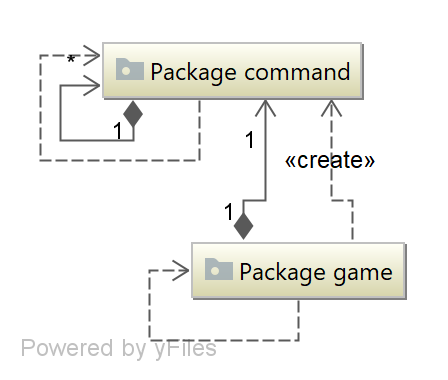
\includegraphics[width=10cm]{Source/Module/Control/Control.png}
\caption{UML Diagram of Module Control}
\label{Control}
\end{figure}

\subsubsection{Package Board}
The Board subsystem of the Model contains the classes which represent the data and state of the Codenames game. This includes classes for game objects such as Card, Board, KeyCard, Clue, and CardType. The subsystem also contains classes which are used to initialize these game objects. The GameManager class includes references to the game objects being played with, and the Players playing the game. The GameManager also contains methods which modify the game state by making players take turns. The Controller's Commands to the Model contain function calls to the GameManager class.

\paragraph{Detailed Design Diagram}\mbox{}
\begin{figure}[H]
\centering
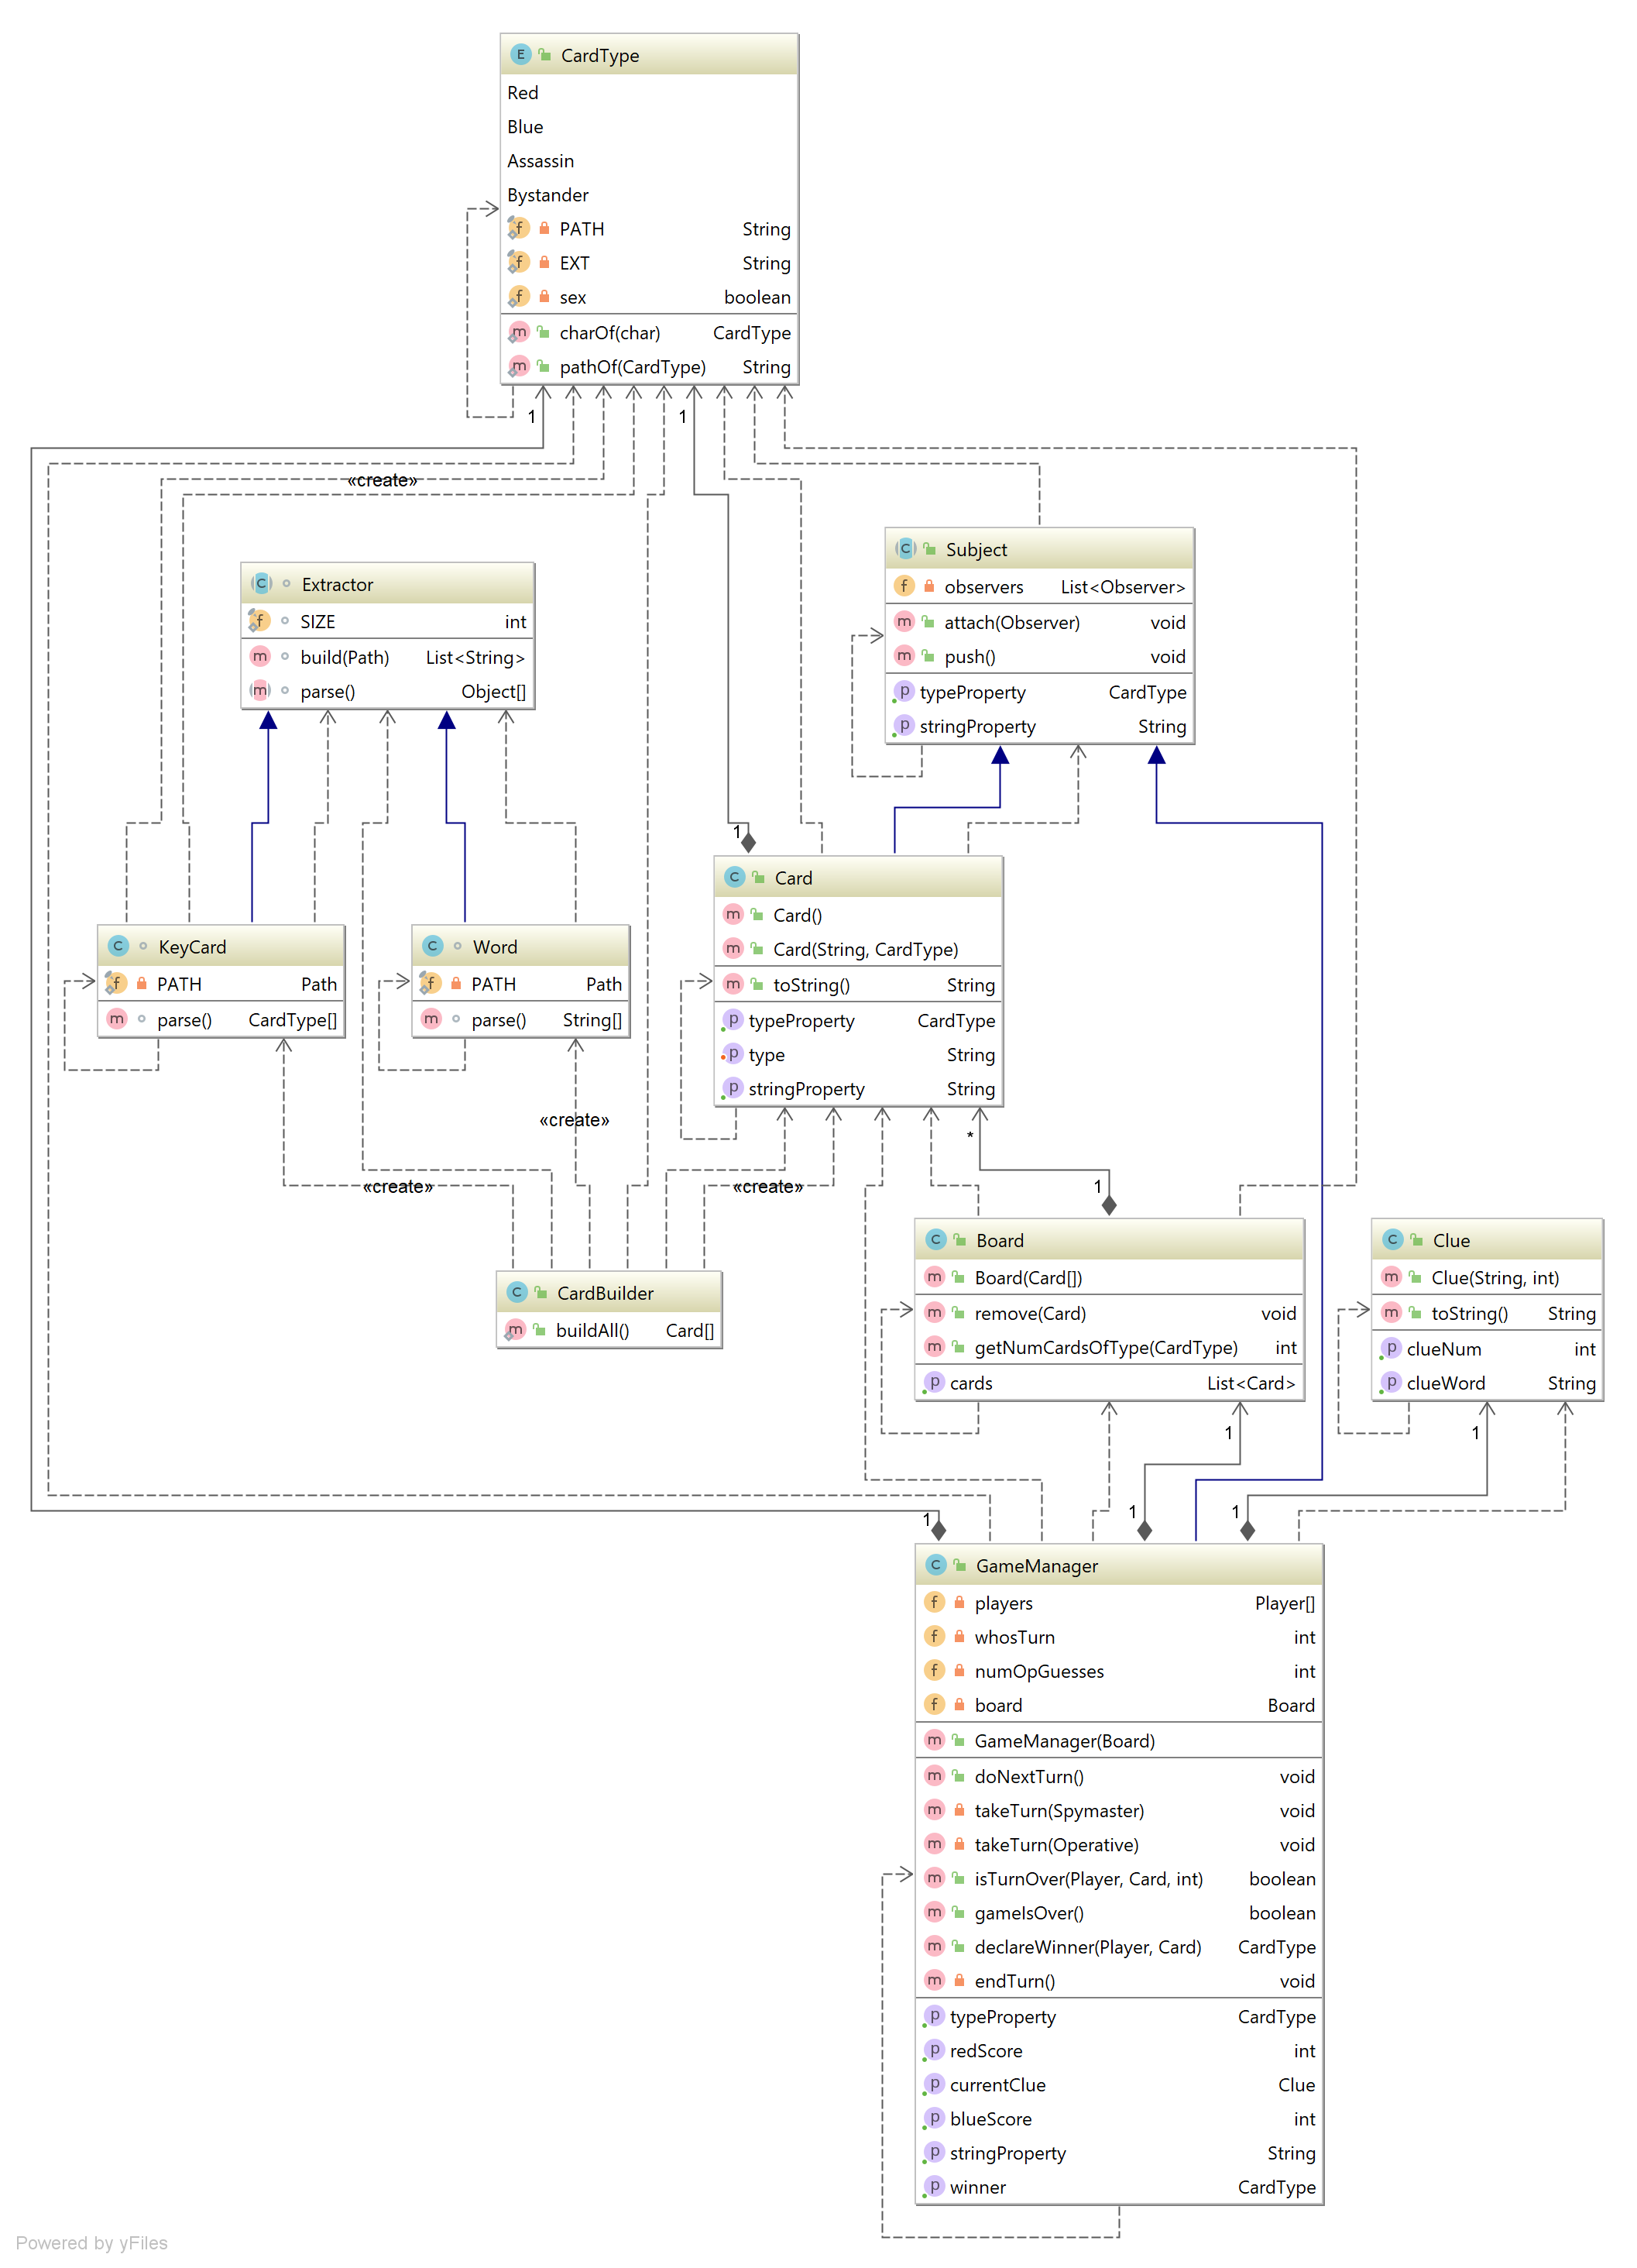
\includegraphics[width=8cm]{Source/Module/Model/Board/Model_Board.png}
\caption{UML Diagram of Package Board in Module Model}
\end{figure}

\paragraph{Class Bipartite}\mbox{}
\begin{tabularx}{\textwidth}{|c||l|p{2.75cm}|l|X|}
    \hline
    \cellcolor{lightgray}Class Name & \multicolumn{4}{X|}{Bipartite}\\
    \hline
    \cellcolor{lightgray}Inherits From & \multicolumn{4}{X|}{None}\\
    \hline
    \cellcolor{lightgray}Description & \multicolumn{4}{p{12cm}|}{Creates a bipartite graph showing the relation between words and clues.}\\
    \hline\hline
    
    \cellcolor{lightgray}Attributes & \cellcolor{lightgray}Visibility & \cellcolor{lightgray}Data type & \cellcolor{lightgray}Name & \cellcolor{lightgray}Description\\\cline{2-5}
    \cellcolor{lightgray} & Private & HashMultiMap \textlangle{}String, String\textrangle{} & wordsToClues & The map from words to clues.\\
    \hline
    \cellcolor{lightgray} & Private & HashMultiMap \textlangle{}String, String\textrangle{} & cluesToWords & The map from clues to words. (One clue can be associated with multiple words)\\
    \hline\hline
    
    \cellcolor{lightgray}Methods & \cellcolor{lightgray}Visibility & \multicolumn{2}{l|}{\cellcolor{lightgray}Method Name} & \cellcolor{lightgray}Description\\\cline{2-5}
    \cellcolor{lightgray} & Public & \multicolumn{2}{l|}{Bipartite(Board board)} & Constructor; creates empty hashMultiMaps and sets them to the board's variables, then processes them.\\
    \hline
    \cellcolor{lightgray} & Private & \multicolumn{2}{l|}{processCards(Board board)} & Creates a bipartite graph with only the words on the current board.\\
    \hline
    \cellcolor{lightgray} & Public & \multicolumn{2}{l|}{getWordsToClues()} & Returns the hash map that contains the mapping of words to clues.\\
    \hline
    \cellcolor{lightgray} & Public & \multicolumn{2}{l|}{getCluesToWords()} & Returns the hash map that contains the mapping of clues to words.\\
    \hline
    \cellcolor{lightgray} & Public & \multicolumn{2}{l|}{getClue(String cardWord)} & Returns a string representation of a clue.\\
    \hline
    \cellcolor{lightgray} & Public & \multicolumn{2}{l|}{removeWord(String word)} & Removes a word from the bipartite including its related clues.\\
    \hline
    \cellcolor{lightgray} & Private & \multicolumn{2}{l|}{debug()} & Prints the current status of the bipartite.\\
    \hline
    
\end{tabularx}
\paragraph{Class Board}\mbox{}
 \begin{tabularx}{\textwidth}{|c||l|l|l|X|}
    \hline
    \cellcolor{lightgray}Class Name & \multicolumn{4}{X|}{Board}\\
    \hline
    \cellcolor{lightgray}Inherits From & \multicolumn{4}{X|}{None}\\
    \hline
    \cellcolor{lightgray}Description & \multicolumn{4}{p{12cm}|}{The board stores the set of code name Cards on the board, which have not yet been guessed.}\\
    \hline\hline
    \cellcolor{lightgray}Attributes & \cellcolor{lightgray}Visibility & \cellcolor{lightgray}Data type & \cellcolor{lightgray}Name & \cellcolor{lightgray}Description\\\cline{2-5}
    \cellcolor{lightgray} & Private & List of Cards & cards & Holds the set of Cards that have not yet been guessed by Operatives\\
    \hline\hline
    
    \cellcolor{lightgray}Methods & \cellcolor{lightgray}Visibility & \multicolumn{2}{l|}{\cellcolor{lightgray}Method Name} & \cellcolor{lightgray}Description\\\cline{2-5}
    \cellcolor{lightgray} & Public & \multicolumn{2}{l|}{Board(Card[] cards)} & Initializes the board with a list of cards.\\
    \hline
    \cellcolor{lightgray} & Public & \multicolumn{2}{l|}{remove(Card c)} & Remove the specified card from the set of unchosen cards.\\
    \hline
    \cellcolor{lightgray} & Public & \multicolumn{2}{l|}{getCards()} & Return all of the unchosen cards still available, as a List.\\
    \hline
    \cellcolor{lightgray} & Public & \multicolumn{2}{X|}{getNumCardsOfType (CardType type)} & Return integer count of the number of unchosen cards left with color specified by variable type.\\
    \hline
\end{tabularx}
\paragraph{Class Card}\mbox{}
\begin{tabularx}{\textwidth}{|c||l|l|l|X|}
    \hline
    \cellcolor{lightgray}Class Name & \multicolumn{4}{X|}{Card}\\
    \hline
    \cellcolor{lightgray}Inherits From & \multicolumn{4}{X|}{Extends Subject}\\
    \hline
    \cellcolor{lightgray}Description & \multicolumn{4}{p{12cm}|}{The Card class represents a single codenames card, and it's true identity (color). It is a subject in the observer pattern, because the view's CardPanes each individually observe a card.}\\
    \hline\hline
    \cellcolor{lightgray}Attributes & \cellcolor{lightgray}Visibility & \cellcolor{lightgray}Data type & \cellcolor{lightgray}Name & \cellcolor{lightgray}Description\\\cline{2-5}
    \cellcolor{lightgray} & Private & String & word & The codename word.\\
    \hline
    \cellcolor{lightgray} & Private & CardType & type & The true identity of the card: Blue, Red, Assassin, or Bystander.\\
    \hline\hline
    \cellcolor{lightgray}Methods & \cellcolor{lightgray}Visibility & \multicolumn{2}{l|}{\cellcolor{lightgray}Method Name} & \cellcolor{lightgray}Description\\\cline{2-5}
    \cellcolor{lightgray} & Public & \multicolumn{2}{l|}{Card()} & Default constructor; initializes word and type to null.\\
    \hline
    \cellcolor{lightgray} & Public & \multicolumn{2}{X|}{Card (String word, CardType type)} & Constructor.\\
    \hline
    \cellcolor{lightgray} & Public & \multicolumn{2}{l|}{setType(String word)} & Sets the codename on this card. \\
    \hline
    \cellcolor{lightgray} & Public & \multicolumn{2}{l|}{toString()} & Returns the codename. Could be changed to return color and word. \\
    \hline
    \cellcolor{lightgray} & Public & \multicolumn{2}{l|}{getStringProperty()} & Returns the codename. This overrides a method of Subject. \\
    \hline
    \cellcolor{lightgray} & Public & \multicolumn{2}{l|}{getTypeProperty()} & Returns the cards true identity (color). This overrides a method of Subject. \\
    \hline
\end{tabularx}
\paragraph{Class Extractor}\mbox{}
\begin{tabularx}{\textwidth}{|c||l|l|l|X|}
    \hline
    \cellcolor{lightgray}Class Name & \multicolumn{4}{X|}{Extractor}\\
    \hline
    \cellcolor{lightgray}Inherits From & \multicolumn{4}{X|}{None}\\
    \hline
    \cellcolor{lightgray}Description & \multicolumn{4}{p{12cm}|}{Abstract class extractor abstracts the process of ingesting 25 random lines of a file. This process is done in creating the KeyCard from the database of keycards, and for choosing 25 codenames.}\\
    \hline\hline
    \cellcolor{lightgray}Attributes & \cellcolor{lightgray}Visibility & \cellcolor{lightgray}Data type & \cellcolor{lightgray}Name & \cellcolor{lightgray}Description\\\cline{2-5}
    \cellcolor{lightgray} & Private & final int & SIZE & The number of cards in a board. 25.\\
    \hline\hline
    \cellcolor{lightgray}Methods & \cellcolor{lightgray}Visibility & \multicolumn{2}{l|}{\cellcolor{lightgray}Method Name} & \cellcolor{lightgray}Description\\\cline{2-5}
    \cellcolor{lightgray} & Public & \multicolumn{2}{l|}{build(Path path)} & Returns every line of the file at Path path as a list.\\
    \hline
    \cellcolor{lightgray} & abstract & \multicolumn{2}{l|}{parse()} & To be overridden by any Extractor, to return a list of whatever objects the class is creating from the data it extracts.\\
    \hline
\end{tabularx}
\paragraph{Class Word}\mbox{}
\begin{tabularx}{\textwidth}{|c||l|l|l|X|}
    \hline
    \cellcolor{lightgray}Class Name & \multicolumn{4}{X|}{Word}\\
    \hline
    \cellcolor{lightgray}Inherits From & \multicolumn{4}{X|}{extends Extractor}\\
    \hline
    \cellcolor{lightgray}Description & \multicolumn{4}{p{12cm}|}{Extracts words from a file and returns the first 25.}\\
    \hline\hline
    \cellcolor{lightgray}Attributes & \cellcolor{lightgray}Visibility & \cellcolor{lightgray}Data type & \cellcolor{lightgray}Name & \cellcolor{lightgray}Description\\\cline{2-5}
    \cellcolor{lightgray} & Private & final Path & PATH & The path to the .txt file containing the codenames.\\
    \hline\hline
    \cellcolor{lightgray}Methods & \cellcolor{lightgray}Visibility & \multicolumn{2}{l|}{\cellcolor{lightgray}Method Name} & \cellcolor{lightgray}Description\\\cline{2-5}
    \hline
    \cellcolor{lightgray} & Public & \multicolumn{2}{l|}{parse()} & Calls build() and returns only the first 25 elements of the randomly ordered list of Strings (to be codenames).\\
    \hline
\end{tabularx}
\paragraph{Class KeyCard}\mbox{}

\begin{tabularx}{\textwidth}{|c||l|l|l|X|}
    \hline
    \cellcolor{lightgray}Class Name & \multicolumn{4}{X|}{KeyCard}\\
    \hline
    \cellcolor{lightgray}Inherits From & \multicolumn{4}{X|}{extends Extractor}\\
    \hline
    \cellcolor{lightgray}Description & \multicolumn{4}{p{12cm}|}{Extracts all of the data representing KeyCards from a text file, then chooses a random one and parses it into a List of CardTypes.}\\
    \hline\hline
    
    \cellcolor{lightgray}Methods & \cellcolor{lightgray}Visibility & \multicolumn{2}{l|}{\cellcolor{lightgray}Method Name} & \cellcolor{lightgray}Description\\\cline{2-5}
    \hline
    \cellcolor{lightgray} & Public & \multicolumn{2}{l|}{parse()} & Uses build() to get the possible Key Cards in a random order, then takes the first one and maps each character to a CardType to create a list of CardTypes.\\
    \hline
\end{tabularx}
\paragraph{Class CardBuilder}\mbox{}
\begin{tabularx}{\textwidth}{|c||l|l|l|X|}
    \hline
    \cellcolor{lightgray}Class Name & \multicolumn{4}{X|}{CardBuilder}\\
    \hline
    \cellcolor{lightgray}Inherits From & \multicolumn{4}{X|}{None}\\
    \hline
    \cellcolor{lightgray}Description & \multicolumn{4}{p{12cm}|}{Creates an array of Card objects based on a random selection of 25 words and a key card.}\\
    \hline\hline
    
    \cellcolor{lightgray}Methods & \cellcolor{lightgray}Visibility & \multicolumn{2}{l|}{\cellcolor{lightgray}Method Name} & \cellcolor{lightgray}Description\\\cline{2-5}
    \cellcolor{lightgray} & Public & \multicolumn{2}{l|}{buildAll()} & Use the KeyCard and Word classes to create an array of 25 Cards (the core of the board).\\
    \hline
    
\end{tabularx}
\paragraph{Class CardType}\mbox{}
\begin{tabularx}{\textwidth}{|c||l|l|l|X|}
    \hline
    \cellcolor{lightgray}Class Name & \multicolumn{4}{X|}{CardType}\\
    \hline
    \cellcolor{lightgray}Inherits From & \multicolumn{4}{X|}{None}\\
    \hline
    \cellcolor{lightgray}Description & \multicolumn{4}{p{12cm}|}{An enum type which represents the possible colours of a card on a Key Card. Blue, Red, Assassin, or Bystander. Can also be used for team colour.}\\

    \hline\hline
    \cellcolor{lightgray}Attributes & \cellcolor{lightgray}Visibility & \cellcolor{lightgray}Data type & \cellcolor{lightgray}Name & \cellcolor{lightgray}Description\\\cline{2-5}
    \cellcolor{lightgray} & Private & String & PATH & The path to the images used by the GUI to represent the colours on the board.\\
    \hline    
    \cellcolor{lightgray} & Private & String & EXT & The file extension of the images used by the GUI to represent the colours on the board.\\
    \hline    
    \cellcolor{lightgray} & Private & boolean & sex & For the GUI, some cards should be displayed as male spys and some should be female.\\
    \hline\hline
    \cellcolor{lightgray}Methods & \cellcolor{lightgray}Visibility & \multicolumn{2}{l|}{\cellcolor{lightgray}Method Name} & \cellcolor{lightgray}Description\\\cline{2-5}
    \hline
    \cellcolor{lightgray} & Public & \multicolumn{2}{l|}{charOf(char arg)} & Each CardType is represented in the database as a character in a String. charOf returns the CardType represented by a character. B is Blue, R is Red, Y is Bystander, A is Assassin.\\
    \hline
    \cellcolor{lightgray} & Public & \multicolumn{2}{l|}{pathOf(CardType type)} & Returns the path to the image which can be used to display this colour on the board GUI.\\
    \hline
\end{tabularx}
\paragraph{Class Clue}\mbox{}

\begin{tabularx}{\textwidth}{|c||l|l|l|X|}
    \hline
    \cellcolor{lightgray}Class Name & \multicolumn{4}{X|}{Clue}\\
    \hline
    \cellcolor{lightgray}Inherits From & \multicolumn{4}{X|}{None}\\
    \hline
    \cellcolor{lightgray}Description & \multicolumn{4}{p{12cm}|}{Represents a Clue given by a SpyMaster. Keeps track of the clue word and the number of associated cards. }\\

    \hline\hline
    \cellcolor{lightgray}Attributes & \cellcolor{lightgray}Visibility & \cellcolor{lightgray}Data type & \cellcolor{lightgray}Name & \cellcolor{lightgray}Description\\\cline{2-5}
    \cellcolor{lightgray} & Private & String & clueWord & The word part of the clue.\\
    \hline    
    \cellcolor{lightgray} & Private & int & clueNum & The number part of the clue. Should represent the number of Cards associated with the word. \\
    \hline\hline
    \cellcolor{lightgray}Methods & \cellcolor{lightgray}Visibility & \multicolumn{2}{l|}{\cellcolor{lightgray}Method Name} & \cellcolor{lightgray}Description\\\cline{2-5}
    \hline
    \cellcolor{lightgray} & Public & \multicolumn{2}{X|}{Clue(String clueWord, int clueNum)} & Constructor.\\
    \hline
    \cellcolor{lightgray} & Public & \multicolumn{2}{l|}{getClueWord()} & Getter for the clue word. \\
    \hline
    \cellcolor{lightgray} & Public & \multicolumn{2}{l|}{getClueNum()} & Getter for the clue number. \\
    \hline
    \cellcolor{lightgray} & Public & \multicolumn{2}{l|}{toString()} & Clue represented as a string. Could be "Word:Num".\\
    \hline
\end{tabularx}
\paragraph{Class Constants}\mbox{}
\begin{tabularx}{\textwidth}{|c||l|l|l|X|}
    \hline
    \cellcolor{lightgray}Class Name & \multicolumn{4}{X|}{Constants}\\
    \hline
    \cellcolor{lightgray}Inherits From & \multicolumn{4}{X|}{None}\\
    \hline
    \cellcolor{lightgray}Description & \multicolumn{4}{p{12cm}|}{Stores any constants used across classes}\\
    \hline\hline
    \cellcolor{lightgray}Attributes & \cellcolor{lightgray}Visibility & \cellcolor{lightgray}Data type & \cellcolor{lightgray}Name & \cellcolor{lightgray}Description\\\cline{2-5}
    \cellcolor{lightgray} & Public & Path & WORDS\textunderscore{}PATH & Path to the words file; used for debug.\\
    \hline    
    \cellcolor{lightgray} & Public & boolean & DEBUG & Debug mode. True.\\
    \hline
\end{tabularx}
\paragraph{Class Subject}\mbox{}
\begin{tabularx}{\textwidth}{|c||l|l|l|X|}
    \hline
    \cellcolor{lightgray}Class Name & \multicolumn{4}{X|}{Subject}\\
    \hline
    \cellcolor{lightgray}Inherits From & \multicolumn{4}{X|}{None}\\
    \hline
    \cellcolor{lightgray}Description & \multicolumn{4}{p{12cm}|}{Part of the Observer pattern. Classes which are to be observable (the subjects) extend this class.}\\
    \hline\hline
    
    \cellcolor{lightgray}Attributes & \cellcolor{lightgray}Visibility & \cellcolor{lightgray}Data type & \cellcolor{lightgray}Name & \cellcolor{lightgray}Description\\\cline{2-5}
    \cellcolor{lightgray} & Private & List of Observers & observers & The set of Observers observing this subject.\\ 
    \hline\hline
    
    \cellcolor{lightgray}Methods & \cellcolor{lightgray}Visibility & \multicolumn{2}{l|}{\cellcolor{lightgray}Method Name} & \cellcolor{lightgray}Description\\\cline{2-5}
    \hline
    \cellcolor{lightgray} & Public & \multicolumn{2}{l|}{attach(Observer observer)} & Adds observer to this Subject's list of observers.\\
    \hline
    \cellcolor{lightgray} & Public & \multicolumn{2}{l|}{push()} & Notify all observerrs that the state of this Subject has changed. \\
    \hline
    \cellcolor{lightgray} & Public & \multicolumn{2}{l|}{getStringProperty()} & Abstract method to be overridden by all Subjects. This is a way for Observers to get state information from the Subject, as a String. \\
    \hline
    \cellcolor{lightgray} & Public & \multicolumn{2}{l|}{getTypeProperty()} & Abstract method to be overridden by all Subjects. This is a way for Observers to get state information from the Subject in the form of a CardType (a color).\\
    \hline
\end{tabularx}
\paragraph{Class GameManager}\mbox{}
\begin{tabularx}{\textwidth}{|c||l|l|l|X|}
    \hline
    \cellcolor{lightgray}Class Name & \multicolumn{4}{X|}{GameManager}\\
    \hline
    \cellcolor{lightgray}Inherits From & \multicolumn{4}{X|}{None}\\
    \hline
    \cellcolor{lightgray}Description & \multicolumn{4}{p{12cm}|}{Keeps track of the games state, including the players, current turn, and current clue. Allows manipulation of game state by initiating the next turn. }\\

    \hline\hline
    \cellcolor{lightgray}Attributes & \cellcolor{lightgray}Visibility & \cellcolor{lightgray}Data type & \cellcolor{lightgray}Name & \cellcolor{lightgray}Description\\\cline{2-5}
    \cellcolor{lightgray} & Private & Player[] & players & Array of players participating in the game. Should be 4 players, in order of when they will take their turn. So Red Spy, Red Op, Blue Spy, Blue Op.\\ 
    \hline
    \cellcolor{lightgray} & Private & int & whosTurn & Index into players to keep track of whos turn it currently is.\\ 
    \hline
    \cellcolor{lightgray} & Private & CardType & winningTeam & Holds the colour of the winning team. Not set if nobody has won yet.\\ 
    \hline
    \cellcolor{lightgray} & Private & Clue & currentClue & Reference to the clue given by the team who is currently taking their turn. \\ 
    \hline
    \cellcolor{lightgray} & Private & int & numOpGuesses & Keeps track of how many guesses the operative has made so far in their turn, as the game must enforce a limit.\\ 
    \hline
    \cellcolor{lightgray} & Private & Board & board & Reference to the Board object the game is being played on. \\ 
    \hline
    \cellcolor{lightgray} & Private & Bipartite & bipartite & Shows the relationship between words and clues. \\ 
    \hline\hline
    
    \cellcolor{lightgray}Methods & \cellcolor{lightgray}Visibility & \multicolumn{2}{l|}{\cellcolor{lightgray}Method Name} & \cellcolor{lightgray}Description\\\cline{2-5}
    \hline
    \cellcolor{lightgray} & Public & \multicolumn{2}{l|}{GameManager(Board board)} & Constructor. Start a game with the board.\\
    \hline
    \cellcolor{lightgray} & Public & \multicolumn{2}{l|}{doNextTurn()} & Make the game run the next turn, changing the state of the game.\\
    \hline
    \cellcolor{lightgray} & Private & \multicolumn{2}{l|}{
    takeTurn(Spymaster p)} & Used by doNextTurn(), if the current player is a Spymaster. Makes the Spymaster take its turn. \\
    \hline
    \cellcolor{lightgray} & Private & \multicolumn{2}{l|}{
    takeTurn(Operative p)} & Used by doNextTurn(), if the current player is an Operative. Makes the Operative take its turn. \\
    \hline
    \cellcolor{lightgray} & Public & \multicolumn{2}{X|}{isTurnOver(Player p, Card guess, int clueNum)} & Tells whether or not the current turn should end based on current state information given. \\
    \hline
    \cellcolor{lightgray} & Public & \multicolumn{2}{X|}{gameIsOver()} & Returns true if a winning team has been determined. \\
    \hline
    \cellcolor{lightgray} & Public & \multicolumn{2}{X|}{declareWinner(Player lastPlayer, Card lastGuess)} & Determines the winner based on the last player's team and what card they last guessed. \\
    \hline
    \cellcolor{lightgray} & Public & \multicolumn{2}{X|}{endTurn()} & Ends the turn and resets the number of guesses. \\
    \hline
    \cellcolor{lightgray} & Public & \multicolumn{2}{X|}{getBlueScore()} & Returns the blue team's current score. \\
    \hline
    \cellcolor{lightgray} & Public & \multicolumn{2}{X|}{getRedScore()} & Returns the red team's current score. \\
    \hline
    \cellcolor{lightgray} & Public & \multicolumn{2}{X|}{getWinner()} & Returns the winning team. \\
    \hline
    \cellcolor{lightgray} & Public & \multicolumn{2}{X|}{getCurrentClue()} & Returns the current given clue. \\
    \hline
    \cellcolor{lightgray} & Public & \multicolumn{2}{X|}{getStringProperty()} & Returns either the current clue or a game over message, depending on current game state. \\
    \hline
    \cellcolor{lightgray} & Public & \multicolumn{2}{X|}{getTypeProperty()} & Returns either the team whose turn it is, or the winning team, depending on game state. \\
    \hline
\end{tabularx}
\paragraph{Class JSONProcessor}\mbox{}
\begin{tabularx}{\textwidth}{|c||l|l|l|X|}
    \hline
    \cellcolor{lightgray}Class Name & \multicolumn{4}{X|}{JSONProcessor}\\
    \hline
    \cellcolor{lightgray}Inherits From & \multicolumn{4}{X|}{None}\\
    \hline
    \cellcolor{lightgray}Description & \multicolumn{4}{p{12cm}|}{Processes a .json file and return a JSON object. Using Simple JSON library}\\
    \hline\hline
    
    \cellcolor{lightgray}Methods & \cellcolor{lightgray}Visibility & \multicolumn{2}{l|}{\cellcolor{lightgray}Method Name} & \cellcolor{lightgray}Description\\\cline{2-5}
    \hline
    \cellcolor{lightgray} & Public & \multicolumn{2}{l|}{ProcessCurrentJSON()} & Processes the current .json file defined in Constants.\\
    \hline
    \cellcolor{lightgray} & Public & \multicolumn{2}{l|}{ProcessCustomJSON(Path path)} & Process any kind of .json file\\
    \hline
    \cellcolor{lightgray} & Public & \multicolumn{2}{l|}{ProcessJSON(Path path)} & Process .json object. If the specified file does not exist, the program will terminate and display the error\\
    \hline
\end{tabularx}
\subsubsection{Package Board}
The Board subsystem of the Model contains the classes which represent the data and state of the Codenames game. This includes classes for game objects such as Card, Board, KeyCard, Clue, and CardType. The subsystem also contains classes which are used to initialize these game objects. The GameManager class includes references to the game objects being played with, and the Players playing the game. The GameManager also contains methods which modify the game state by making players take turns. The Controller's Commands to the Model contain function calls to the GameManager class.

\paragraph{Detailed Design Diagram}\mbox{}
\begin{figure}[H]
\centering
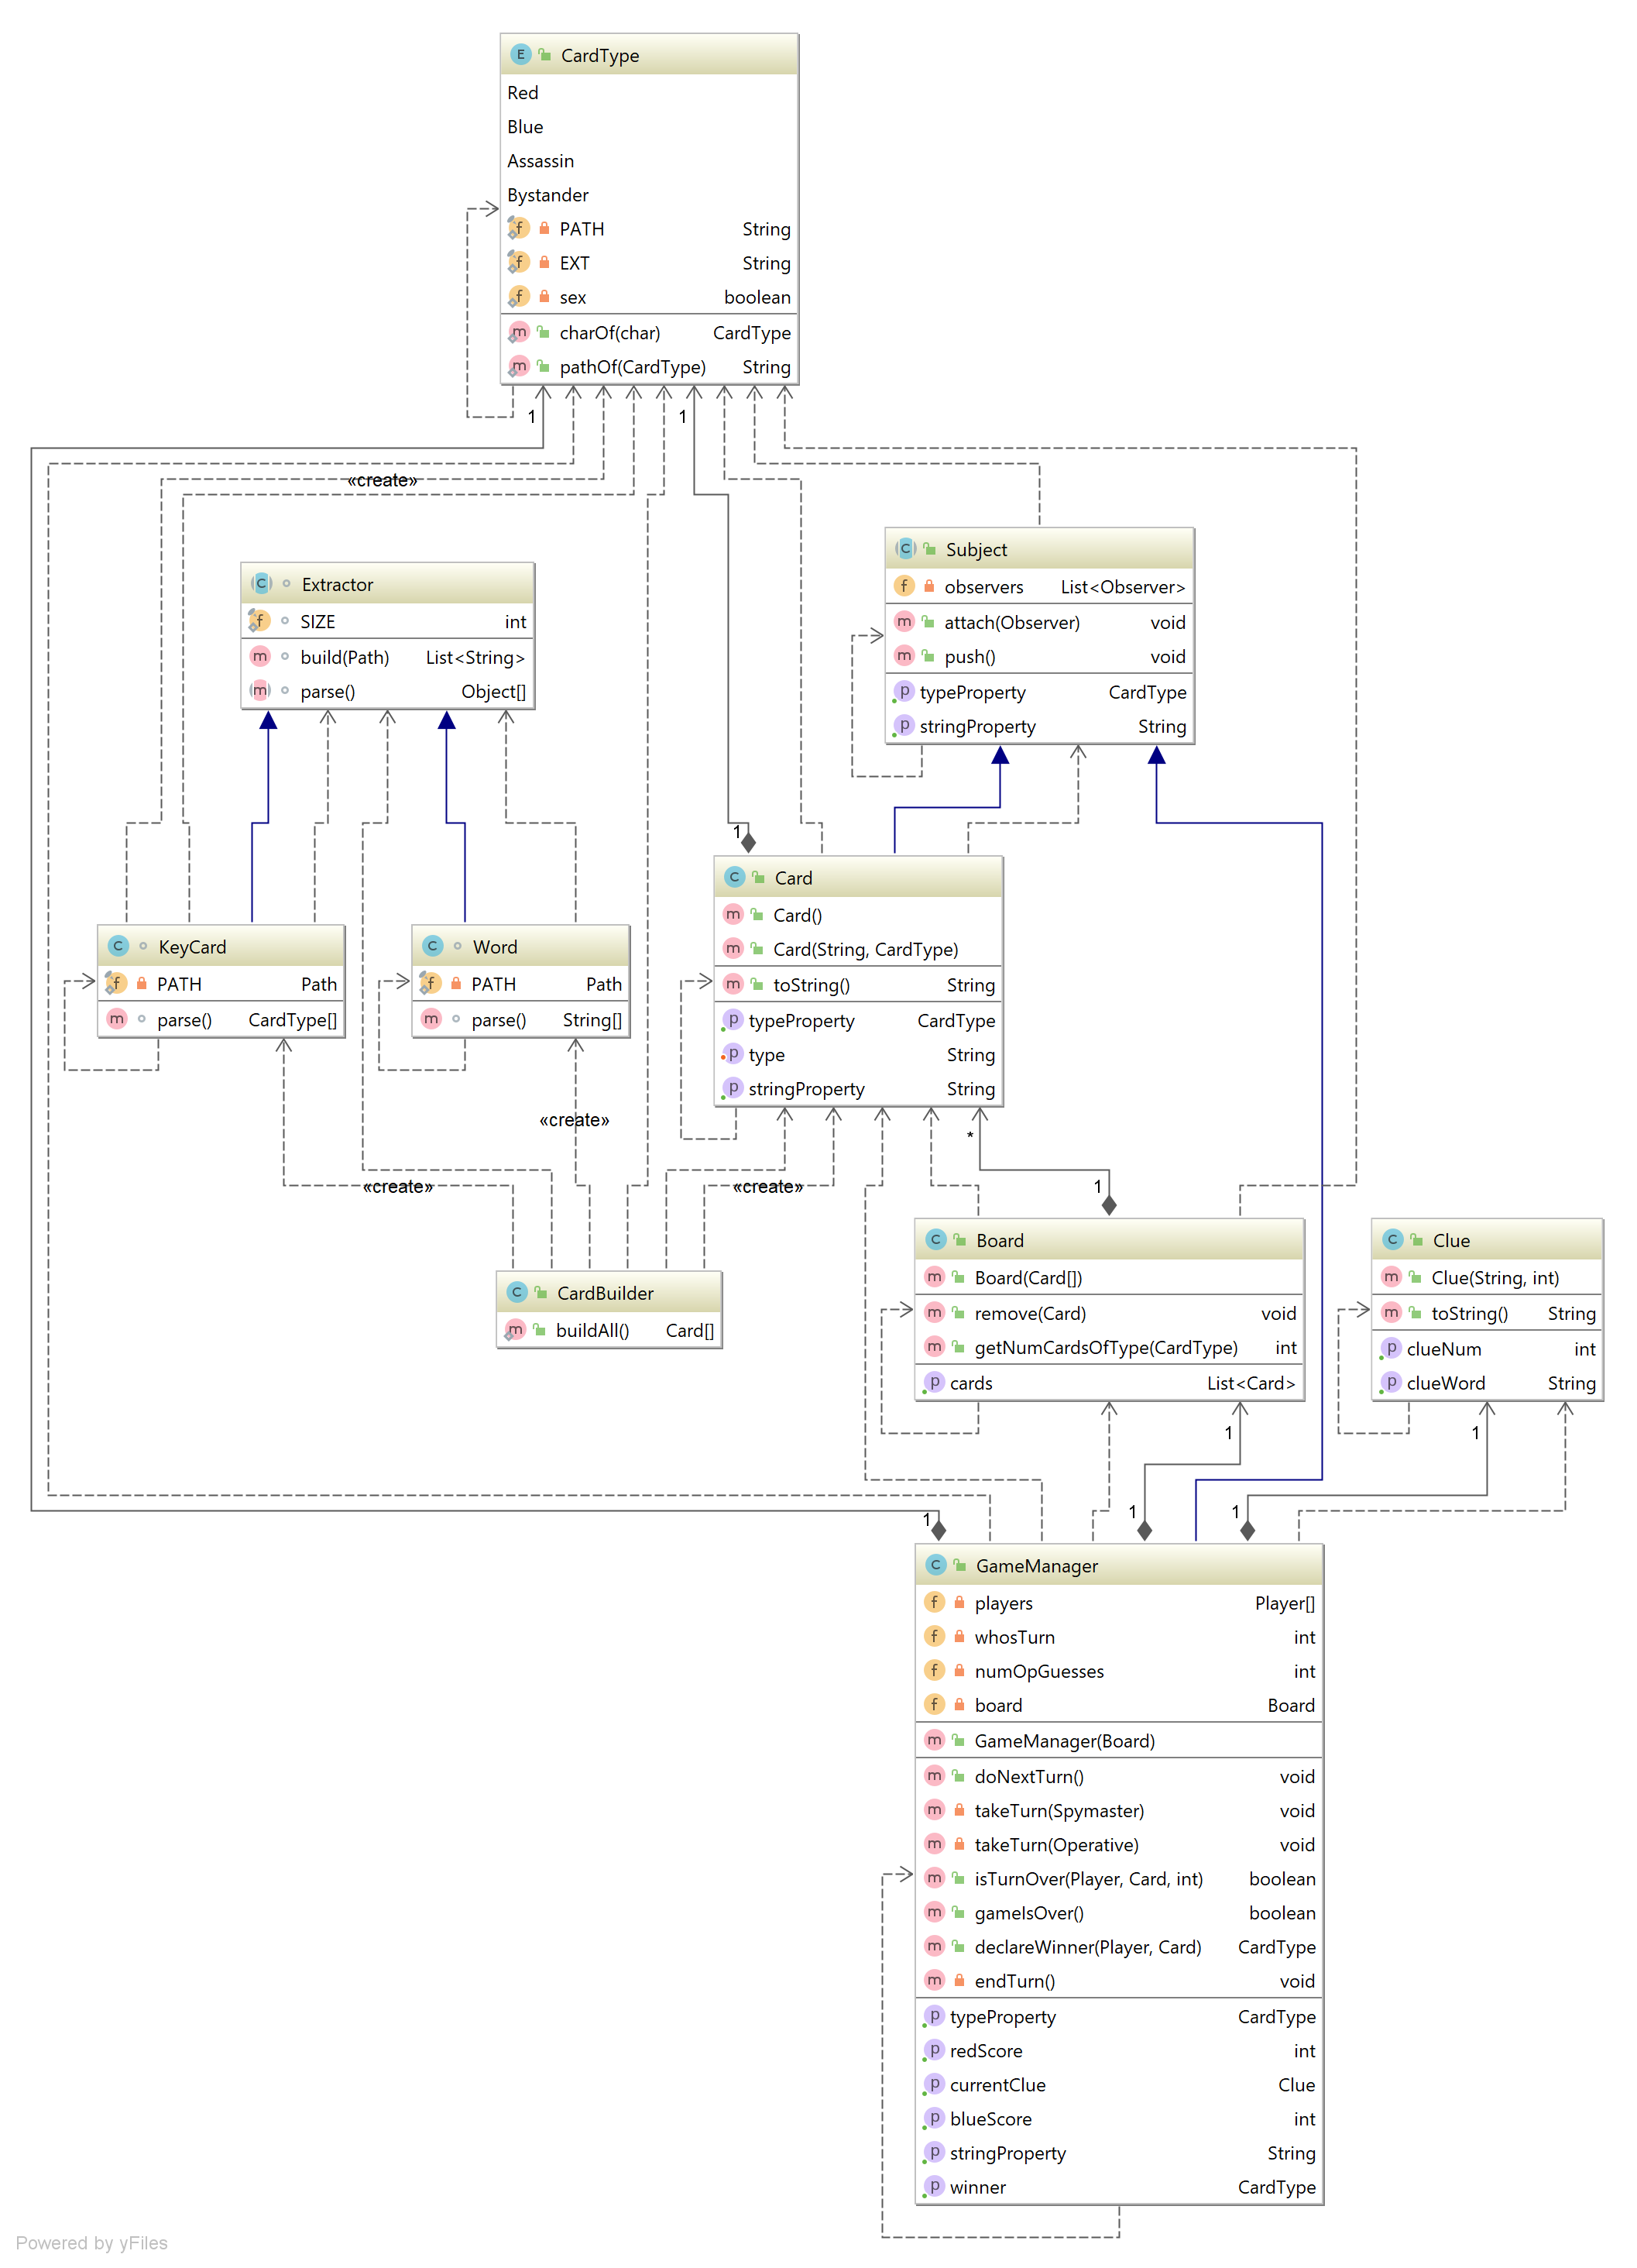
\includegraphics[width=8cm]{Source/Module/Model/Board/Model_Board.png}
\caption{UML Diagram of Package Board in Module Model}
\end{figure}

\paragraph{Class Bipartite}\mbox{}
\begin{tabularx}{\textwidth}{|c||l|p{2.75cm}|l|X|}
    \hline
    \cellcolor{lightgray}Class Name & \multicolumn{4}{X|}{Bipartite}\\
    \hline
    \cellcolor{lightgray}Inherits From & \multicolumn{4}{X|}{None}\\
    \hline
    \cellcolor{lightgray}Description & \multicolumn{4}{p{12cm}|}{Creates a bipartite graph showing the relation between words and clues.}\\
    \hline\hline
    
    \cellcolor{lightgray}Attributes & \cellcolor{lightgray}Visibility & \cellcolor{lightgray}Data type & \cellcolor{lightgray}Name & \cellcolor{lightgray}Description\\\cline{2-5}
    \cellcolor{lightgray} & Private & HashMultiMap \textlangle{}String, String\textrangle{} & wordsToClues & The map from words to clues.\\
    \hline
    \cellcolor{lightgray} & Private & HashMultiMap \textlangle{}String, String\textrangle{} & cluesToWords & The map from clues to words. (One clue can be associated with multiple words)\\
    \hline\hline
    
    \cellcolor{lightgray}Methods & \cellcolor{lightgray}Visibility & \multicolumn{2}{l|}{\cellcolor{lightgray}Method Name} & \cellcolor{lightgray}Description\\\cline{2-5}
    \cellcolor{lightgray} & Public & \multicolumn{2}{l|}{Bipartite(Board board)} & Constructor; creates empty hashMultiMaps and sets them to the board's variables, then processes them.\\
    \hline
    \cellcolor{lightgray} & Private & \multicolumn{2}{l|}{processCards(Board board)} & Creates a bipartite graph with only the words on the current board.\\
    \hline
    \cellcolor{lightgray} & Public & \multicolumn{2}{l|}{getWordsToClues()} & Returns the hash map that contains the mapping of words to clues.\\
    \hline
    \cellcolor{lightgray} & Public & \multicolumn{2}{l|}{getCluesToWords()} & Returns the hash map that contains the mapping of clues to words.\\
    \hline
    \cellcolor{lightgray} & Public & \multicolumn{2}{l|}{getClue(String cardWord)} & Returns a string representation of a clue.\\
    \hline
    \cellcolor{lightgray} & Public & \multicolumn{2}{l|}{removeWord(String word)} & Removes a word from the bipartite including its related clues.\\
    \hline
    \cellcolor{lightgray} & Private & \multicolumn{2}{l|}{debug()} & Prints the current status of the bipartite.\\
    \hline
    
\end{tabularx}
\paragraph{Class Board}\mbox{}
 \begin{tabularx}{\textwidth}{|c||l|l|l|X|}
    \hline
    \cellcolor{lightgray}Class Name & \multicolumn{4}{X|}{Board}\\
    \hline
    \cellcolor{lightgray}Inherits From & \multicolumn{4}{X|}{None}\\
    \hline
    \cellcolor{lightgray}Description & \multicolumn{4}{p{12cm}|}{The board stores the set of code name Cards on the board, which have not yet been guessed.}\\
    \hline\hline
    \cellcolor{lightgray}Attributes & \cellcolor{lightgray}Visibility & \cellcolor{lightgray}Data type & \cellcolor{lightgray}Name & \cellcolor{lightgray}Description\\\cline{2-5}
    \cellcolor{lightgray} & Private & List of Cards & cards & Holds the set of Cards that have not yet been guessed by Operatives\\
    \hline\hline
    
    \cellcolor{lightgray}Methods & \cellcolor{lightgray}Visibility & \multicolumn{2}{l|}{\cellcolor{lightgray}Method Name} & \cellcolor{lightgray}Description\\\cline{2-5}
    \cellcolor{lightgray} & Public & \multicolumn{2}{l|}{Board(Card[] cards)} & Initializes the board with a list of cards.\\
    \hline
    \cellcolor{lightgray} & Public & \multicolumn{2}{l|}{remove(Card c)} & Remove the specified card from the set of unchosen cards.\\
    \hline
    \cellcolor{lightgray} & Public & \multicolumn{2}{l|}{getCards()} & Return all of the unchosen cards still available, as a List.\\
    \hline
    \cellcolor{lightgray} & Public & \multicolumn{2}{X|}{getNumCardsOfType (CardType type)} & Return integer count of the number of unchosen cards left with color specified by variable type.\\
    \hline
\end{tabularx}
\paragraph{Class Card}\mbox{}
\begin{tabularx}{\textwidth}{|c||l|l|l|X|}
    \hline
    \cellcolor{lightgray}Class Name & \multicolumn{4}{X|}{Card}\\
    \hline
    \cellcolor{lightgray}Inherits From & \multicolumn{4}{X|}{Extends Subject}\\
    \hline
    \cellcolor{lightgray}Description & \multicolumn{4}{p{12cm}|}{The Card class represents a single codenames card, and it's true identity (color). It is a subject in the observer pattern, because the view's CardPanes each individually observe a card.}\\
    \hline\hline
    \cellcolor{lightgray}Attributes & \cellcolor{lightgray}Visibility & \cellcolor{lightgray}Data type & \cellcolor{lightgray}Name & \cellcolor{lightgray}Description\\\cline{2-5}
    \cellcolor{lightgray} & Private & String & word & The codename word.\\
    \hline
    \cellcolor{lightgray} & Private & CardType & type & The true identity of the card: Blue, Red, Assassin, or Bystander.\\
    \hline\hline
    \cellcolor{lightgray}Methods & \cellcolor{lightgray}Visibility & \multicolumn{2}{l|}{\cellcolor{lightgray}Method Name} & \cellcolor{lightgray}Description\\\cline{2-5}
    \cellcolor{lightgray} & Public & \multicolumn{2}{l|}{Card()} & Default constructor; initializes word and type to null.\\
    \hline
    \cellcolor{lightgray} & Public & \multicolumn{2}{X|}{Card (String word, CardType type)} & Constructor.\\
    \hline
    \cellcolor{lightgray} & Public & \multicolumn{2}{l|}{setType(String word)} & Sets the codename on this card. \\
    \hline
    \cellcolor{lightgray} & Public & \multicolumn{2}{l|}{toString()} & Returns the codename. Could be changed to return color and word. \\
    \hline
    \cellcolor{lightgray} & Public & \multicolumn{2}{l|}{getStringProperty()} & Returns the codename. This overrides a method of Subject. \\
    \hline
    \cellcolor{lightgray} & Public & \multicolumn{2}{l|}{getTypeProperty()} & Returns the cards true identity (color). This overrides a method of Subject. \\
    \hline
\end{tabularx}
\paragraph{Class Extractor}\mbox{}
\begin{tabularx}{\textwidth}{|c||l|l|l|X|}
    \hline
    \cellcolor{lightgray}Class Name & \multicolumn{4}{X|}{Extractor}\\
    \hline
    \cellcolor{lightgray}Inherits From & \multicolumn{4}{X|}{None}\\
    \hline
    \cellcolor{lightgray}Description & \multicolumn{4}{p{12cm}|}{Abstract class extractor abstracts the process of ingesting 25 random lines of a file. This process is done in creating the KeyCard from the database of keycards, and for choosing 25 codenames.}\\
    \hline\hline
    \cellcolor{lightgray}Attributes & \cellcolor{lightgray}Visibility & \cellcolor{lightgray}Data type & \cellcolor{lightgray}Name & \cellcolor{lightgray}Description\\\cline{2-5}
    \cellcolor{lightgray} & Private & final int & SIZE & The number of cards in a board. 25.\\
    \hline\hline
    \cellcolor{lightgray}Methods & \cellcolor{lightgray}Visibility & \multicolumn{2}{l|}{\cellcolor{lightgray}Method Name} & \cellcolor{lightgray}Description\\\cline{2-5}
    \cellcolor{lightgray} & Public & \multicolumn{2}{l|}{build(Path path)} & Returns every line of the file at Path path as a list.\\
    \hline
    \cellcolor{lightgray} & abstract & \multicolumn{2}{l|}{parse()} & To be overridden by any Extractor, to return a list of whatever objects the class is creating from the data it extracts.\\
    \hline
\end{tabularx}
\paragraph{Class Word}\mbox{}
\begin{tabularx}{\textwidth}{|c||l|l|l|X|}
    \hline
    \cellcolor{lightgray}Class Name & \multicolumn{4}{X|}{Word}\\
    \hline
    \cellcolor{lightgray}Inherits From & \multicolumn{4}{X|}{extends Extractor}\\
    \hline
    \cellcolor{lightgray}Description & \multicolumn{4}{p{12cm}|}{Extracts words from a file and returns the first 25.}\\
    \hline\hline
    \cellcolor{lightgray}Attributes & \cellcolor{lightgray}Visibility & \cellcolor{lightgray}Data type & \cellcolor{lightgray}Name & \cellcolor{lightgray}Description\\\cline{2-5}
    \cellcolor{lightgray} & Private & final Path & PATH & The path to the .txt file containing the codenames.\\
    \hline\hline
    \cellcolor{lightgray}Methods & \cellcolor{lightgray}Visibility & \multicolumn{2}{l|}{\cellcolor{lightgray}Method Name} & \cellcolor{lightgray}Description\\\cline{2-5}
    \hline
    \cellcolor{lightgray} & Public & \multicolumn{2}{l|}{parse()} & Calls build() and returns only the first 25 elements of the randomly ordered list of Strings (to be codenames).\\
    \hline
\end{tabularx}
\paragraph{Class KeyCard}\mbox{}

\begin{tabularx}{\textwidth}{|c||l|l|l|X|}
    \hline
    \cellcolor{lightgray}Class Name & \multicolumn{4}{X|}{KeyCard}\\
    \hline
    \cellcolor{lightgray}Inherits From & \multicolumn{4}{X|}{extends Extractor}\\
    \hline
    \cellcolor{lightgray}Description & \multicolumn{4}{p{12cm}|}{Extracts all of the data representing KeyCards from a text file, then chooses a random one and parses it into a List of CardTypes.}\\
    \hline\hline
    
    \cellcolor{lightgray}Methods & \cellcolor{lightgray}Visibility & \multicolumn{2}{l|}{\cellcolor{lightgray}Method Name} & \cellcolor{lightgray}Description\\\cline{2-5}
    \hline
    \cellcolor{lightgray} & Public & \multicolumn{2}{l|}{parse()} & Uses build() to get the possible Key Cards in a random order, then takes the first one and maps each character to a CardType to create a list of CardTypes.\\
    \hline
\end{tabularx}
\paragraph{Class CardBuilder}\mbox{}
\begin{tabularx}{\textwidth}{|c||l|l|l|X|}
    \hline
    \cellcolor{lightgray}Class Name & \multicolumn{4}{X|}{CardBuilder}\\
    \hline
    \cellcolor{lightgray}Inherits From & \multicolumn{4}{X|}{None}\\
    \hline
    \cellcolor{lightgray}Description & \multicolumn{4}{p{12cm}|}{Creates an array of Card objects based on a random selection of 25 words and a key card.}\\
    \hline\hline
    
    \cellcolor{lightgray}Methods & \cellcolor{lightgray}Visibility & \multicolumn{2}{l|}{\cellcolor{lightgray}Method Name} & \cellcolor{lightgray}Description\\\cline{2-5}
    \cellcolor{lightgray} & Public & \multicolumn{2}{l|}{buildAll()} & Use the KeyCard and Word classes to create an array of 25 Cards (the core of the board).\\
    \hline
    
\end{tabularx}
\paragraph{Class CardType}\mbox{}
\begin{tabularx}{\textwidth}{|c||l|l|l|X|}
    \hline
    \cellcolor{lightgray}Class Name & \multicolumn{4}{X|}{CardType}\\
    \hline
    \cellcolor{lightgray}Inherits From & \multicolumn{4}{X|}{None}\\
    \hline
    \cellcolor{lightgray}Description & \multicolumn{4}{p{12cm}|}{An enum type which represents the possible colours of a card on a Key Card. Blue, Red, Assassin, or Bystander. Can also be used for team colour.}\\

    \hline\hline
    \cellcolor{lightgray}Attributes & \cellcolor{lightgray}Visibility & \cellcolor{lightgray}Data type & \cellcolor{lightgray}Name & \cellcolor{lightgray}Description\\\cline{2-5}
    \cellcolor{lightgray} & Private & String & PATH & The path to the images used by the GUI to represent the colours on the board.\\
    \hline    
    \cellcolor{lightgray} & Private & String & EXT & The file extension of the images used by the GUI to represent the colours on the board.\\
    \hline    
    \cellcolor{lightgray} & Private & boolean & sex & For the GUI, some cards should be displayed as male spys and some should be female.\\
    \hline\hline
    \cellcolor{lightgray}Methods & \cellcolor{lightgray}Visibility & \multicolumn{2}{l|}{\cellcolor{lightgray}Method Name} & \cellcolor{lightgray}Description\\\cline{2-5}
    \hline
    \cellcolor{lightgray} & Public & \multicolumn{2}{l|}{charOf(char arg)} & Each CardType is represented in the database as a character in a String. charOf returns the CardType represented by a character. B is Blue, R is Red, Y is Bystander, A is Assassin.\\
    \hline
    \cellcolor{lightgray} & Public & \multicolumn{2}{l|}{pathOf(CardType type)} & Returns the path to the image which can be used to display this colour on the board GUI.\\
    \hline
\end{tabularx}
\paragraph{Class Clue}\mbox{}

\begin{tabularx}{\textwidth}{|c||l|l|l|X|}
    \hline
    \cellcolor{lightgray}Class Name & \multicolumn{4}{X|}{Clue}\\
    \hline
    \cellcolor{lightgray}Inherits From & \multicolumn{4}{X|}{None}\\
    \hline
    \cellcolor{lightgray}Description & \multicolumn{4}{p{12cm}|}{Represents a Clue given by a SpyMaster. Keeps track of the clue word and the number of associated cards. }\\

    \hline\hline
    \cellcolor{lightgray}Attributes & \cellcolor{lightgray}Visibility & \cellcolor{lightgray}Data type & \cellcolor{lightgray}Name & \cellcolor{lightgray}Description\\\cline{2-5}
    \cellcolor{lightgray} & Private & String & clueWord & The word part of the clue.\\
    \hline    
    \cellcolor{lightgray} & Private & int & clueNum & The number part of the clue. Should represent the number of Cards associated with the word. \\
    \hline\hline
    \cellcolor{lightgray}Methods & \cellcolor{lightgray}Visibility & \multicolumn{2}{l|}{\cellcolor{lightgray}Method Name} & \cellcolor{lightgray}Description\\\cline{2-5}
    \hline
    \cellcolor{lightgray} & Public & \multicolumn{2}{X|}{Clue(String clueWord, int clueNum)} & Constructor.\\
    \hline
    \cellcolor{lightgray} & Public & \multicolumn{2}{l|}{getClueWord()} & Getter for the clue word. \\
    \hline
    \cellcolor{lightgray} & Public & \multicolumn{2}{l|}{getClueNum()} & Getter for the clue number. \\
    \hline
    \cellcolor{lightgray} & Public & \multicolumn{2}{l|}{toString()} & Clue represented as a string. Could be "Word:Num".\\
    \hline
\end{tabularx}
\paragraph{Class Constants}\mbox{}
\begin{tabularx}{\textwidth}{|c||l|l|l|X|}
    \hline
    \cellcolor{lightgray}Class Name & \multicolumn{4}{X|}{Constants}\\
    \hline
    \cellcolor{lightgray}Inherits From & \multicolumn{4}{X|}{None}\\
    \hline
    \cellcolor{lightgray}Description & \multicolumn{4}{p{12cm}|}{Stores any constants used across classes}\\
    \hline\hline
    \cellcolor{lightgray}Attributes & \cellcolor{lightgray}Visibility & \cellcolor{lightgray}Data type & \cellcolor{lightgray}Name & \cellcolor{lightgray}Description\\\cline{2-5}
    \cellcolor{lightgray} & Public & Path & WORDS\textunderscore{}PATH & Path to the words file; used for debug.\\
    \hline    
    \cellcolor{lightgray} & Public & boolean & DEBUG & Debug mode. True.\\
    \hline
\end{tabularx}
\paragraph{Class Subject}\mbox{}
\begin{tabularx}{\textwidth}{|c||l|l|l|X|}
    \hline
    \cellcolor{lightgray}Class Name & \multicolumn{4}{X|}{Subject}\\
    \hline
    \cellcolor{lightgray}Inherits From & \multicolumn{4}{X|}{None}\\
    \hline
    \cellcolor{lightgray}Description & \multicolumn{4}{p{12cm}|}{Part of the Observer pattern. Classes which are to be observable (the subjects) extend this class.}\\
    \hline\hline
    
    \cellcolor{lightgray}Attributes & \cellcolor{lightgray}Visibility & \cellcolor{lightgray}Data type & \cellcolor{lightgray}Name & \cellcolor{lightgray}Description\\\cline{2-5}
    \cellcolor{lightgray} & Private & List of Observers & observers & The set of Observers observing this subject.\\ 
    \hline\hline
    
    \cellcolor{lightgray}Methods & \cellcolor{lightgray}Visibility & \multicolumn{2}{l|}{\cellcolor{lightgray}Method Name} & \cellcolor{lightgray}Description\\\cline{2-5}
    \hline
    \cellcolor{lightgray} & Public & \multicolumn{2}{l|}{attach(Observer observer)} & Adds observer to this Subject's list of observers.\\
    \hline
    \cellcolor{lightgray} & Public & \multicolumn{2}{l|}{push()} & Notify all observerrs that the state of this Subject has changed. \\
    \hline
    \cellcolor{lightgray} & Public & \multicolumn{2}{l|}{getStringProperty()} & Abstract method to be overridden by all Subjects. This is a way for Observers to get state information from the Subject, as a String. \\
    \hline
    \cellcolor{lightgray} & Public & \multicolumn{2}{l|}{getTypeProperty()} & Abstract method to be overridden by all Subjects. This is a way for Observers to get state information from the Subject in the form of a CardType (a color).\\
    \hline
\end{tabularx}
\paragraph{Class GameManager}\mbox{}
\begin{tabularx}{\textwidth}{|c||l|l|l|X|}
    \hline
    \cellcolor{lightgray}Class Name & \multicolumn{4}{X|}{GameManager}\\
    \hline
    \cellcolor{lightgray}Inherits From & \multicolumn{4}{X|}{None}\\
    \hline
    \cellcolor{lightgray}Description & \multicolumn{4}{p{12cm}|}{Keeps track of the games state, including the players, current turn, and current clue. Allows manipulation of game state by initiating the next turn. }\\

    \hline\hline
    \cellcolor{lightgray}Attributes & \cellcolor{lightgray}Visibility & \cellcolor{lightgray}Data type & \cellcolor{lightgray}Name & \cellcolor{lightgray}Description\\\cline{2-5}
    \cellcolor{lightgray} & Private & Player[] & players & Array of players participating in the game. Should be 4 players, in order of when they will take their turn. So Red Spy, Red Op, Blue Spy, Blue Op.\\ 
    \hline
    \cellcolor{lightgray} & Private & int & whosTurn & Index into players to keep track of whos turn it currently is.\\ 
    \hline
    \cellcolor{lightgray} & Private & CardType & winningTeam & Holds the colour of the winning team. Not set if nobody has won yet.\\ 
    \hline
    \cellcolor{lightgray} & Private & Clue & currentClue & Reference to the clue given by the team who is currently taking their turn. \\ 
    \hline
    \cellcolor{lightgray} & Private & int & numOpGuesses & Keeps track of how many guesses the operative has made so far in their turn, as the game must enforce a limit.\\ 
    \hline
    \cellcolor{lightgray} & Private & Board & board & Reference to the Board object the game is being played on. \\ 
    \hline
    \cellcolor{lightgray} & Private & Bipartite & bipartite & Shows the relationship between words and clues. \\ 
    \hline\hline
    
    \cellcolor{lightgray}Methods & \cellcolor{lightgray}Visibility & \multicolumn{2}{l|}{\cellcolor{lightgray}Method Name} & \cellcolor{lightgray}Description\\\cline{2-5}
    \hline
    \cellcolor{lightgray} & Public & \multicolumn{2}{l|}{GameManager(Board board)} & Constructor. Start a game with the board.\\
    \hline
    \cellcolor{lightgray} & Public & \multicolumn{2}{l|}{doNextTurn()} & Make the game run the next turn, changing the state of the game.\\
    \hline
    \cellcolor{lightgray} & Private & \multicolumn{2}{l|}{
    takeTurn(Spymaster p)} & Used by doNextTurn(), if the current player is a Spymaster. Makes the Spymaster take its turn. \\
    \hline
    \cellcolor{lightgray} & Private & \multicolumn{2}{l|}{
    takeTurn(Operative p)} & Used by doNextTurn(), if the current player is an Operative. Makes the Operative take its turn. \\
    \hline
    \cellcolor{lightgray} & Public & \multicolumn{2}{X|}{isTurnOver(Player p, Card guess, int clueNum)} & Tells whether or not the current turn should end based on current state information given. \\
    \hline
    \cellcolor{lightgray} & Public & \multicolumn{2}{X|}{gameIsOver()} & Returns true if a winning team has been determined. \\
    \hline
    \cellcolor{lightgray} & Public & \multicolumn{2}{X|}{declareWinner(Player lastPlayer, Card lastGuess)} & Determines the winner based on the last player's team and what card they last guessed. \\
    \hline
    \cellcolor{lightgray} & Public & \multicolumn{2}{X|}{endTurn()} & Ends the turn and resets the number of guesses. \\
    \hline
    \cellcolor{lightgray} & Public & \multicolumn{2}{X|}{getBlueScore()} & Returns the blue team's current score. \\
    \hline
    \cellcolor{lightgray} & Public & \multicolumn{2}{X|}{getRedScore()} & Returns the red team's current score. \\
    \hline
    \cellcolor{lightgray} & Public & \multicolumn{2}{X|}{getWinner()} & Returns the winning team. \\
    \hline
    \cellcolor{lightgray} & Public & \multicolumn{2}{X|}{getCurrentClue()} & Returns the current given clue. \\
    \hline
    \cellcolor{lightgray} & Public & \multicolumn{2}{X|}{getStringProperty()} & Returns either the current clue or a game over message, depending on current game state. \\
    \hline
    \cellcolor{lightgray} & Public & \multicolumn{2}{X|}{getTypeProperty()} & Returns either the team whose turn it is, or the winning team, depending on game state. \\
    \hline
\end{tabularx}
\paragraph{Class JSONProcessor}\mbox{}
\begin{tabularx}{\textwidth}{|c||l|l|l|X|}
    \hline
    \cellcolor{lightgray}Class Name & \multicolumn{4}{X|}{JSONProcessor}\\
    \hline
    \cellcolor{lightgray}Inherits From & \multicolumn{4}{X|}{None}\\
    \hline
    \cellcolor{lightgray}Description & \multicolumn{4}{p{12cm}|}{Processes a .json file and return a JSON object. Using Simple JSON library}\\
    \hline\hline
    
    \cellcolor{lightgray}Methods & \cellcolor{lightgray}Visibility & \multicolumn{2}{l|}{\cellcolor{lightgray}Method Name} & \cellcolor{lightgray}Description\\\cline{2-5}
    \hline
    \cellcolor{lightgray} & Public & \multicolumn{2}{l|}{ProcessCurrentJSON()} & Processes the current .json file defined in Constants.\\
    \hline
    \cellcolor{lightgray} & Public & \multicolumn{2}{l|}{ProcessCustomJSON(Path path)} & Process any kind of .json file\\
    \hline
    \cellcolor{lightgray} & Public & \multicolumn{2}{l|}{ProcessJSON(Path path)} & Process .json object. If the specified file does not exist, the program will terminate and display the error\\
    \hline
\end{tabularx}